\documentclass{paper}

\usepackage{latexsym}
\usepackage{amssymb}
\usepackage{amsmath}
\usepackage{amsfonts}
\usepackage{verbatim}
\usepackage{listings}
\usepackage{graphicx}
\usepackage{float}

\begin{document}

\section{Implement Gradient Descent}

When testing my gradient descent procedure on the function
\[
f(x, y) = x^2 + y^2,
\]
which has gradient
\[
\nabla f(x, y) = [2x, 2y]
\]
with an initial guess of $(x, y) = (3, 5)$, a step size of $0.1$, and a convergence criterion of $10^{-11}$. it returns an answer of $(x_{min}, y_{min}) = (6.17064209 * 10^{-7},   1.02844035 * 10^{-6})$. By inspection, the actual minimum of $f$ occurs at $(0, 0)$. The gradient descent function was close to the correct answer, and can be made arbitrarily closer by lowering the value of the convergence criterion. The convergence criterion is the threshold value $t$ such that the descent algorithm stops running and returns $g_{i+1}$ when $|f(g_i) - f(g_{i+1})| \le t$, where the $g_j$ are successive guesses as to the vector $(x_{min}, y_{min})$.

If lowering the convergence criterion makes the result closer to the true answer, what about changing the step size and the starting guess? Increasing the step size from $0.1$ reduces the error in the answer, up until the step size is $0.5$ - this also decreases the number of iterations that the algorithm needs to run before converging. When the step size is $0.5$ in this example the answer is exactly correct - the algorithm returns $(0, 0)$; increasing the step size any larger causes the algorithm to overshoot the correct answer by an extremely fast-growing amount, and the number of steps required for convergence is very high. Naturally these numbers are unique to this particular example, but the takeaway is that while having a large step size can increase accuracy and convergence speed up to a point, taking steps that are too large can cause incorrect answers and divergent estimates rather than convergent ones.

Increasing the magnitude of the guess by 10 in this example caused the gradient descent procedure to take 10 more iterations, and the number of iterations continues to grow as the guess becomes further from the answer.

While my gradient descent implementation took between 11 and 55 iterations to converge depending on the parameters, the PyLab function \texttt{fmin\_bfgs} was able to converge in 2 iterations with error on the order of $10^{-15}$ in both $x$ and $y$.

My numerical gradient approximation function using central differences returns very accurate answers. The value of $\nabla f(3, 5)$ should be $(6, 10)$; my approximation function returns $(5.999964969305438, 9.999965300266922)$.

\section{Linear Basis Function Regression}

Computing maximum-likelihood weights, and plotting the polynomials given by those weight vectors for orders 0, 1, 3 and 9, results in the following plots, very similar to the graphs in the Bishop text.

\begin{figure}[H]
	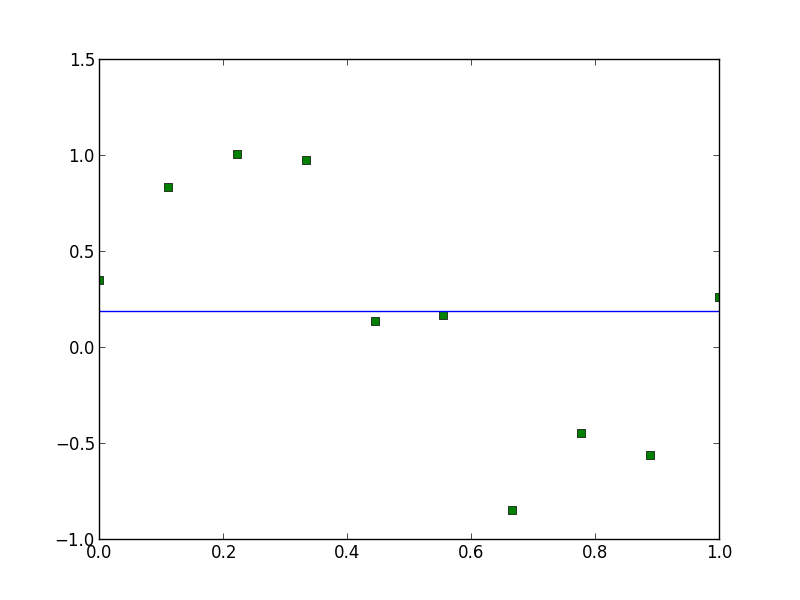
\includegraphics[width=165px]{plot1.png}
	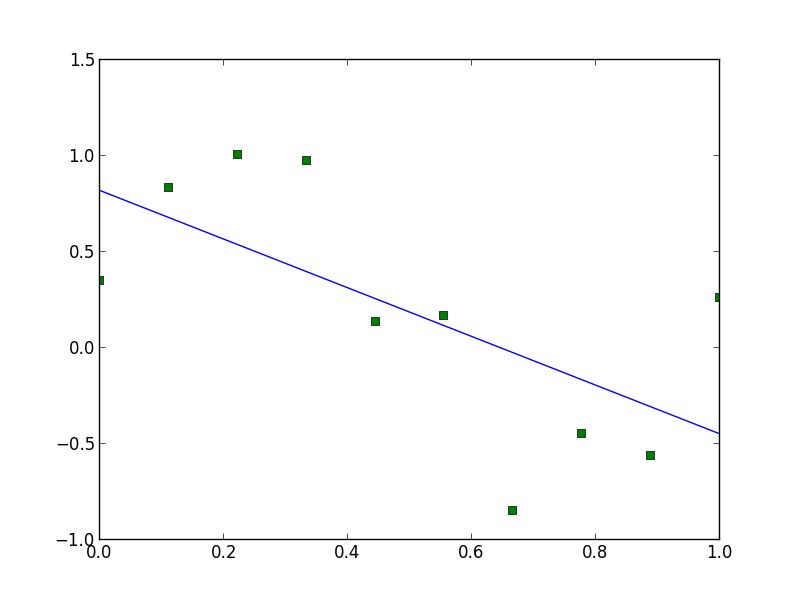
\includegraphics[width=165px]{plot2.png}
	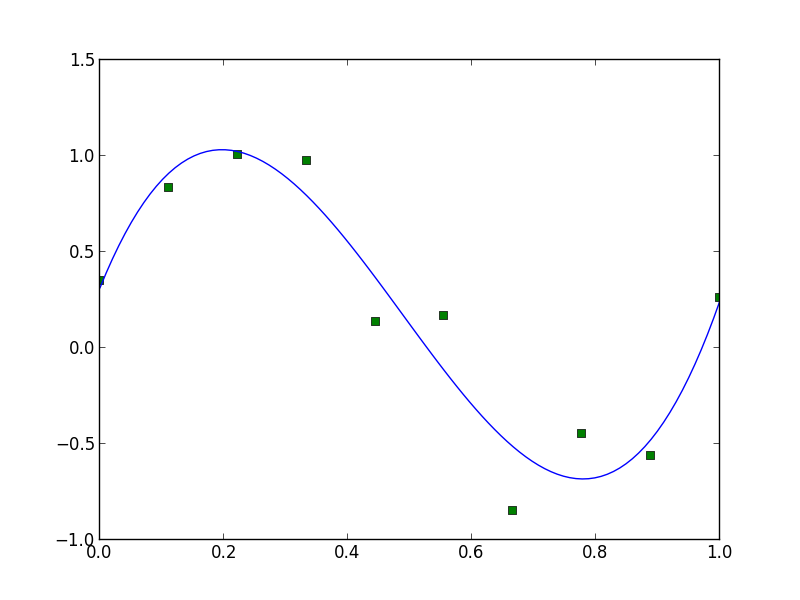
\includegraphics[width=165px]{plot3.png}
	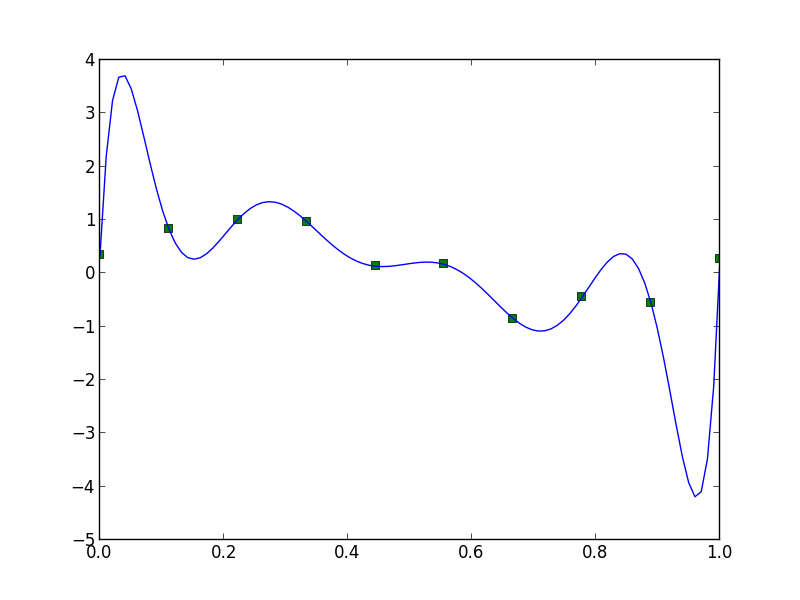
\includegraphics[width=165px]{plot4.png}
	\caption{OLS regression. Fits of order 0 (top left), 1 (top right), 3 (bottom left), 9 (bottom right).}
\end{figure}


When calculating the gradient of the error of these models (evaluated on $w$, the vector of weights), both the analytical function and the numerical gradient function return very similar answers - close to 0. We expect the values to be almost the same, and it makes sense for them both to be close to 0 because the weights were chosen to minimize the error. For examle, in plot number 2 above, the analytically calculated error gradient was $(1.33226763 * 10^{-15}, 1.11022302 * 10^{-15})$, while the numerically calculated gradient was $(4.4408920985006255 * 10^{-11}, 0.0)$.

Setting the step size to 0.01 or 0.02 allows the gradient descent to converge; setting it to 0.1 causes it to wildly diverge. Setting the convergence criterion to $10^{-3}$ causes the algorithm to converge pretty quickly though the fit is not very good. A convergence criterion of $10^{-5}$, however, takes longer but produces a much better fit. PyLab's \texttt{fmin\_bfgs} converges very quickly and produces a good fit.

\section{Ridge Regression}

Upon adding a regularization term to the error function following the ``ridge regression'' technique, overfitting decreased especialy for large values of $M$ (the order of the polynomial used for the fit). Some plots are shown below:

\begin{figure}[H]
	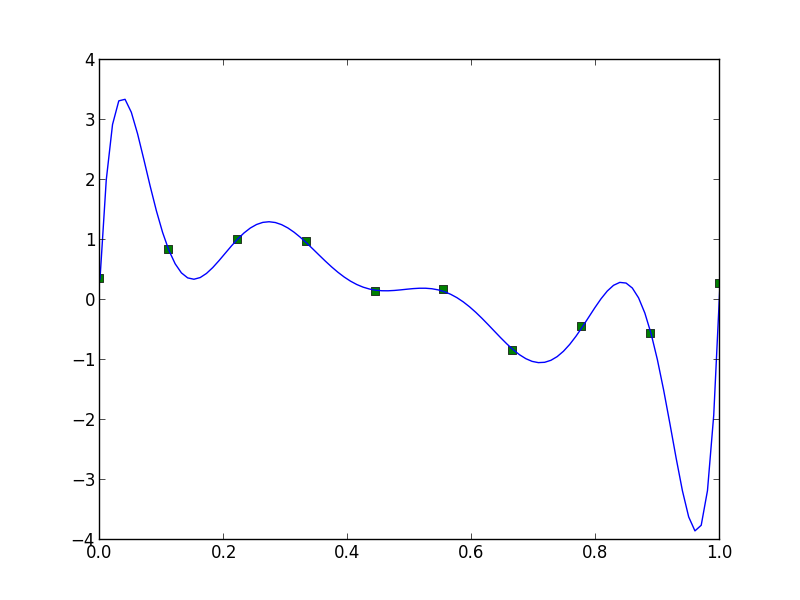
\includegraphics[width=165px]{plot6-underfit-l=0-00000000000001.png}
	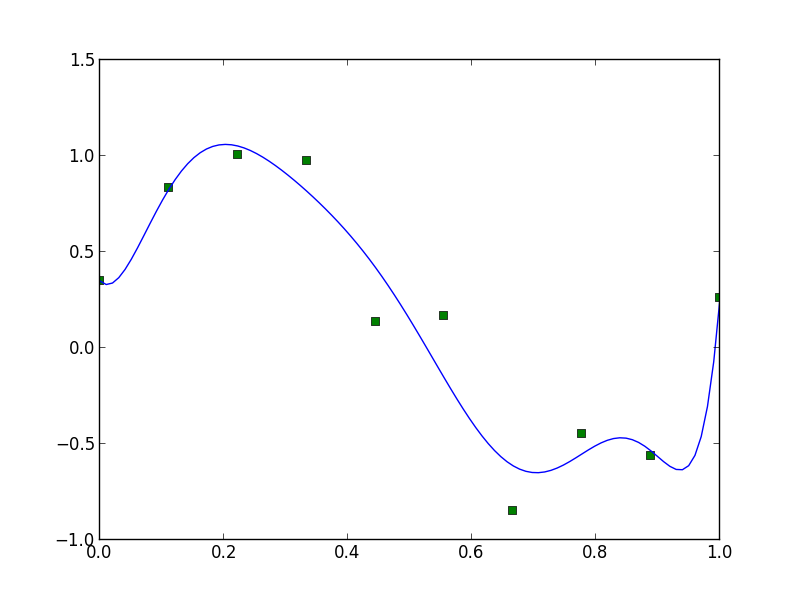
\includegraphics[width=165px]{plot6-underfit-l=0-0000000001.png}
	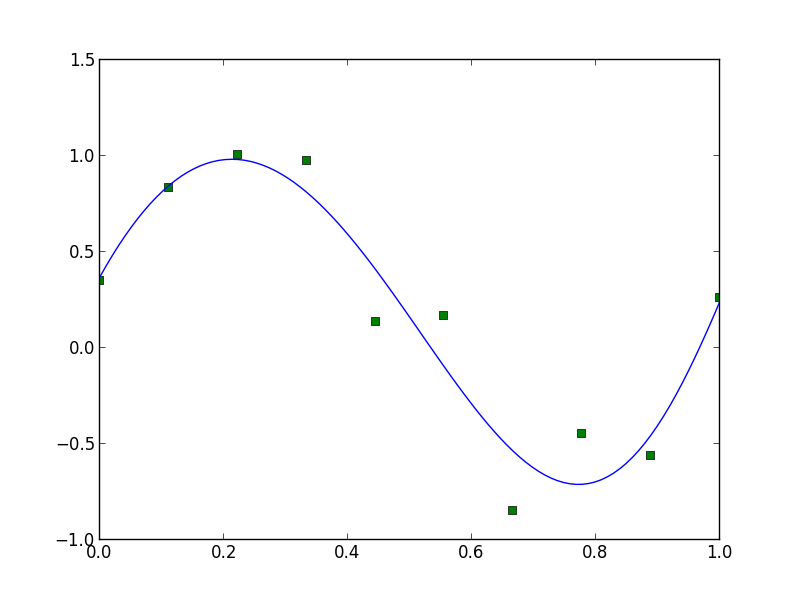
\includegraphics[width=165px]{plot6-underfit-l=0-0001.png}
	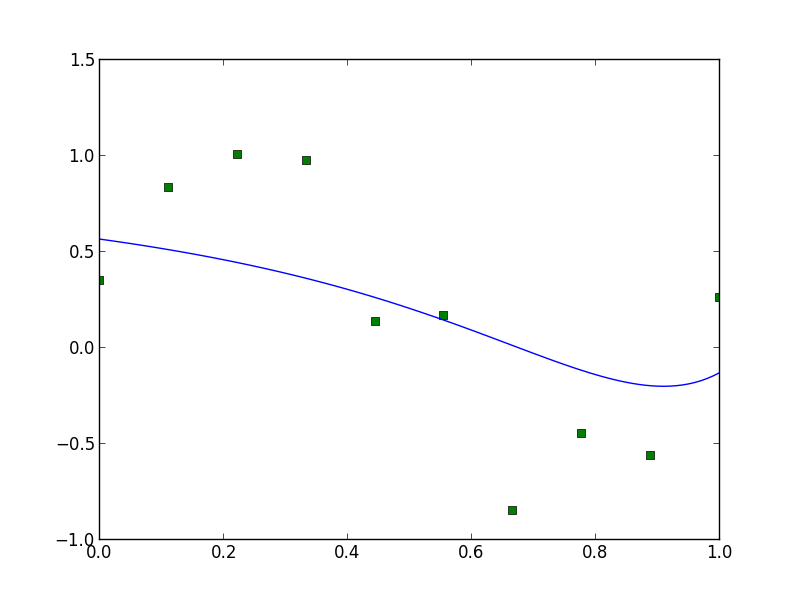
\includegraphics[width=165px]{plot6-underfit-l=1.png}
	\caption{Ridge regression. Fits of order 9 with regularization parameter $10^{-14}$ (top left), $10^{-10}$ (top right), $10^{-4}$ (bottom left), and $1$ (bottom right).}
\end{figure}

Next, I show how the provided training datasets A and B can be used to make predictions about future data (tested against the validation set). I used datasets A and B independently. That is to say, first, using dataset A, I used the closed form solution of ridge regression, substituting particular values of $M$ and $\lambda$, to generate a weight vector $w$ of length $M+1$ (using the $\lambda$ term to combat overfitting). I used the components of the weight vector $w$ as coefficients on a polynomial of order $M$. I took every $X$ value from the validation set, applied the weight vector $w$ as polynomial coefficients to the $X$ values, to calculate predicted $Y$ values. I calculated the total error of these predicted $Y$ values as compared with the actual $Y$ values from the validation set. Doing this repeatedly over a range of values of $M$ and $\lambda$, I was able to select the $(M, \lambda)$ pair that minimized the error. This generated the best model from dataset A, and I was able to repeat that entire process to then generate the best model from dataset B. Each training dataset A and B has its own best fit and its own total error. Dataset A had the better best-fit since the points in dataset A were more representative of the overall shape of the validation set. Dataset B contains an outlier point and so the ridge fit is not as good in the validation set.

For dataset A, the optimal model was $(M, \lambda) = (1, 0)$, which had total error of $1.958$. For dataset B, the optimal model was $(3, 0.1)$, with a total error of $27.117$.

\begin{figure}[H]
	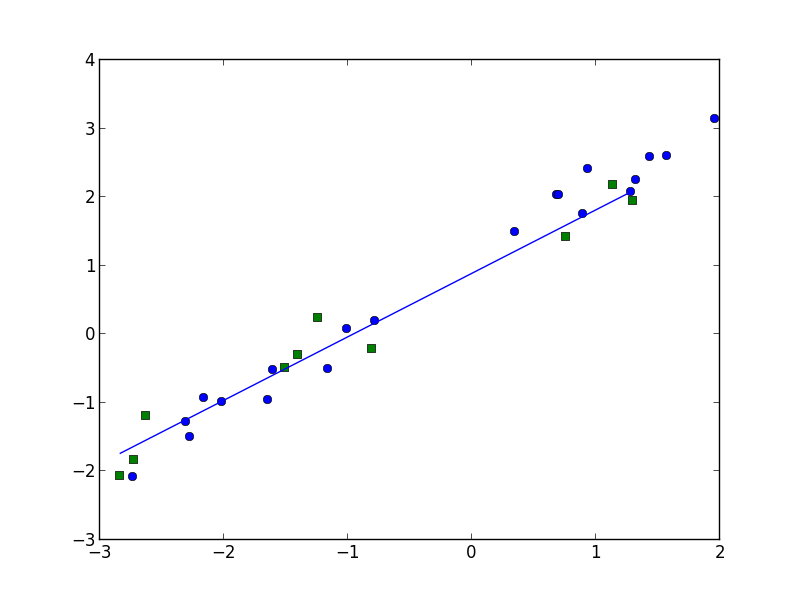
\includegraphics[width=165px]{plot7-regressA-optimal.png}
	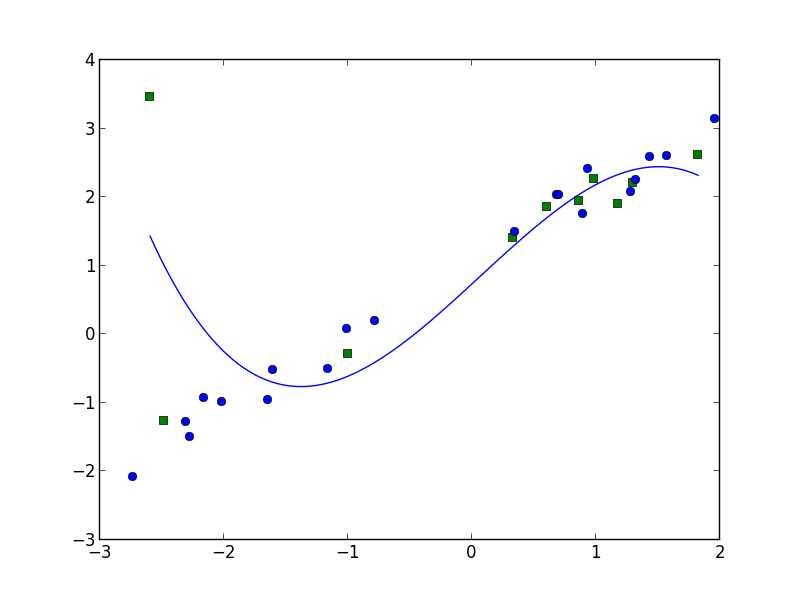
\includegraphics[width=165px]{plot8-regressB-optimal.png}
	\caption{Optimal model selection using ridge regression on datasets A and B. Green squares represent training data points, blue circles represent validation data. Dataset A (left) is fit with $(M, \lambda) = (1, 0)$ and B is fit with $(3, 0.1)$}
\end{figure}

Upon running ridge regression on the blog data, we get a model that is linear in all 280 features. The best fit I found is where $\lambda = 31,750$. But this fit is still not very good - the sum of the squared errors for each prediction is $e = 10,618,658$. Given that the validation set contains $n=10,480$ data points, the average squared error per data point is $\frac{e}{n} = 1013.23$, or an average error of $\sqrt{\frac{e}{n}} = 31.83$ comments per post. Given that the average number of comments per post is $6.824$, an error of $31.83$ comments per post is a lot of error. This error likely comes about because there are some blog posts which have a large number of comments, and that large number of comments could be due to some reason besides the data in the $X$ vectors (i.e. the post got linked to by a very popular news source and suddenly got a huge influx of readers - something like this is not necessarily reflected in the 280 features of the input data). 

I optimized the fit by trying a range of $\lambda$ values in the ridge regression solution on the training data, taking the resulting weight vectors $w$ and trying them on the validation data, then choosing the $\lambda$ value that produced the lowest error. The first range of $\lambda$s I tried were $\lambda_i = 10^{-5}, 10^{-4}, ..., 10^{10}$. I did this for the sake of covering many different orders of magnitude since I had no idea what neighborhood the best choice would be in. From that set I identified the best value $\lambda_j$, then tested a smaller range of $\lambda$s in the range $[\lambda_{j-1}, \lambda_{j+1}]$. From that range, I again selected the best value of $\lambda$. I continued ``zooming in'' on the neighborhood around that optimum until the change in error seemed to be very small. Since we are predicting the number of comments on some blog post, having the error in one prediction change by only $0.01$ is not a big deal at all, especially if the average error is around $30$. This process ought to give as close to the global optimum as desired, since the error as a function of $\lambda$ always seemed to decrease for a little while, then reach some minimum, then begin increasing as $\lambda$ grew from small to large. This was always the case at every range I tested. Plus, it intuitively makes sense that there would not be multiple local minima since $\lambda$ is just a ``smoothing'' or ``damping'' value that transitions the weights between grossly overfit (low $\lambda$) and grossly flat (high $\lambda$), both of which have high error, with a sweet spot somewhere in between depending on the nature of the data.

\section{Generalizations}

Using LAD regression, both datasets A and B produce good fits in the validation set. The total squared error is $0.958$ for dataset A and $1.428$ for dataset B. I computed the squared error only for the purpose of model selection and for comparison with the results of other regression techniques; in the regression itself, naturally I used the LAD error expression and optimized it using gradient descent, with absolute error on the $Y$ values plus the 2-norm of the weight vector. The fit for dataset A is almost the same as it was from ridge regression, however LAD performs much better on dataset B (which contains an outlier) than ridge regression does. This is because squared error penalizes large differences more than absolute error does. So the LAD algorithm is more willing to accept a large error on one outlier point than the normal ridge algorithm is. As such, LAD does not get swayed as much by outliers and fits the validation data better.

\begin{figure}
	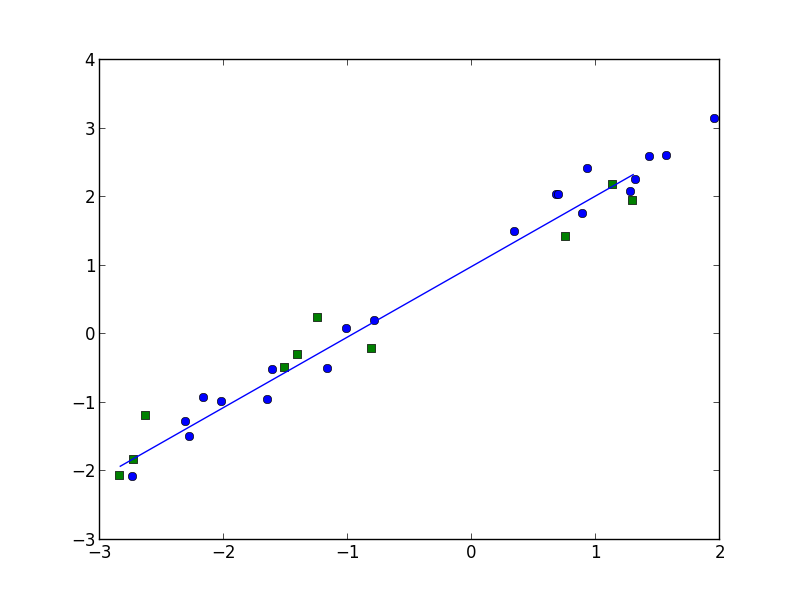
\includegraphics[width=165px]{LAD-A-best-fit.png}
	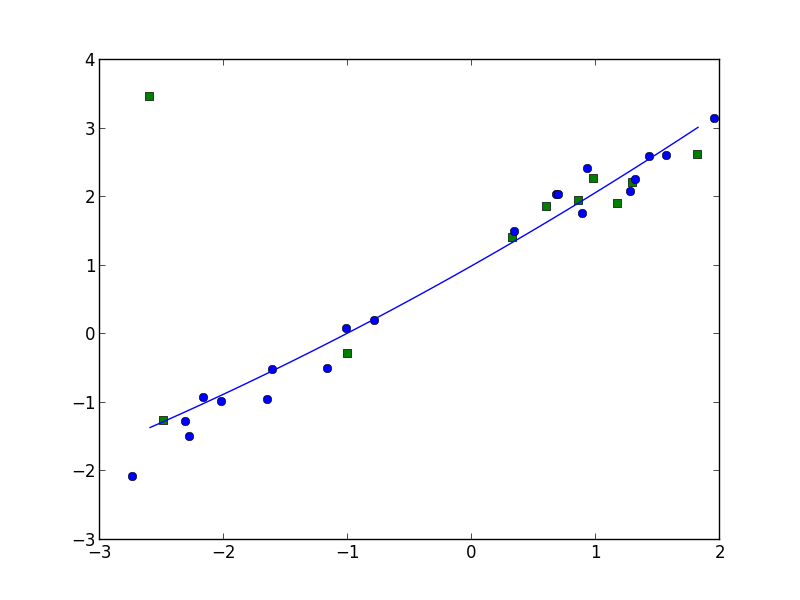
\includegraphics[width=165px]{LAD-B-best-fit.png}
	\caption{Best fit using LAD regression on dataset A (left) and B (right). Green squares are training data and blue circles are validation data.}
\end{figure}

When trained on dataset A, lasso regression chooses a linear model (order $M = 1$) with regularization parameter $\lambda = 0.0$, and returns a weight vector of $(0.890,  0.926)$. The total squared error is $1.958$.
When trained on dataset B, lasso regression chooses a quartic model (order $M = 4$) with regularization parameter $\lambda = 2$, and returns a weight vector of $(1.222, 0.953,  -0.453, -9.841 * 10^{-9},   0.128)$. Lasso regression again has the problem with the outlier in dataset B and hence has a high total squared error ($26.940$). The lasso regularizer tends to drive the least important feature weights to 0, as it has done in this case with the cubic term. 

\begin{figure}
	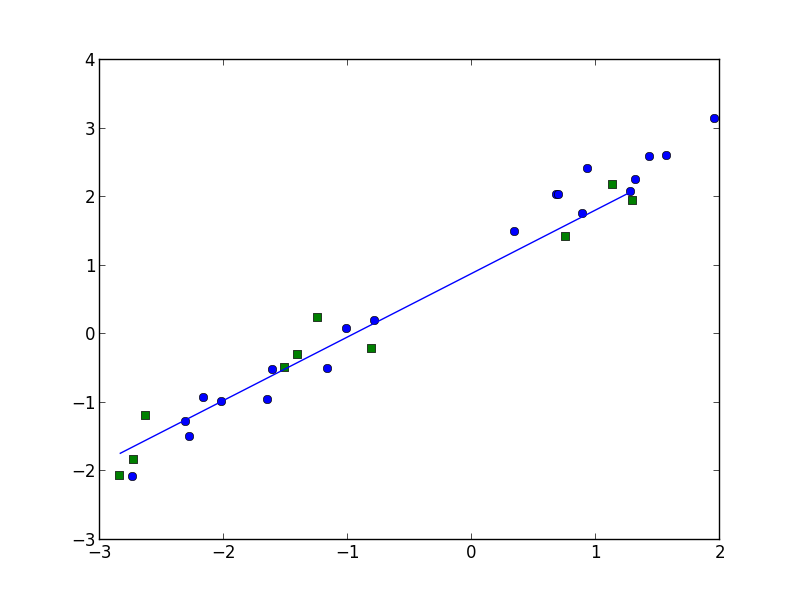
\includegraphics[width=165px]{lasso-A-best-fit.png}
	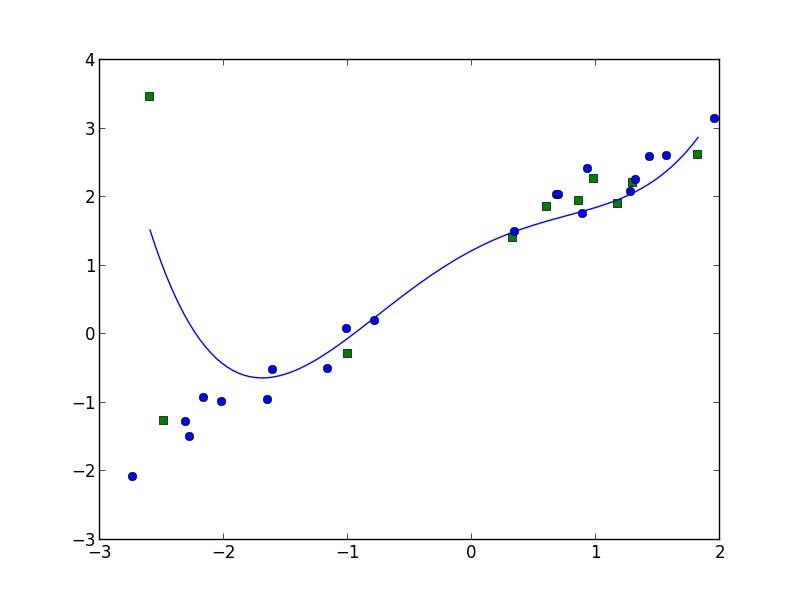
\includegraphics[width=165px]{lasso-B-best-fit.png}
	\caption{Best fit using lasso regression on dataset A (left) and B (right). Green squares are training data and blue circles are validation data.}
\end{figure}

Least absolute deviations is a good approach for decreasing the effect of outlier data points in the training data. The lasso algorithm prevents overfitting by driving more feature weights to 0 as the regularization parameter increases. This is good if you want a model that depends on few parameters.

Using Least Absolute Deviations is almost the same as optimizing weights using the loss function $L(p, a) = |p - a|$. It is not exactly the same because LAD also uses a regularization term. Besides this, there is also the fact that one can use a different error function during regression versus model selection. LAD only necessarily uses this absolute loss function when calculating the weights for a particular model on the training set (i.e. $M$ and $\lambda$ are already chosen). Once the weights are calculated for a particular model, one does not have to necessarily use absolute loss when testing against a validation set for the purpose of model selection (for the same reason that one wouldn't use the regularization term in model selection - regularization is just needed to prevent overfitting to the training data). 

\end{document}

